%\begin{itemize}
%	\setlength\itemsep{1pt}
%	\item Explain in detail what extensibility means.
%	\item Describe the input.
%	\item Describe how we incorporate the auxiliary data into the planner.
%\end{itemize}
Allowing users to upload their own data sets of interests is an important
step towards customization of a trip planner.
We designed a framework where a user can upload auxiliary cost 
metric data (e.g., crime
statistics and pollution data) into the planner,
and the planner will compute an optimal route accordingly.

The user-created data are the auxiliary data that is represented as pairs
of latitude and longitude degrees.
To merge these lat-long pairs into the planner, we performed a neighborhood
search to calculate the total score of auxiliary data for each 
lat-long pair already in our planner.
It might be of strong interest to some user for our planning
system to take care of criminal statistics so that some level of safety
of the resulting routes is guaranteed.
For instance, a user traveling through the downtown area of San Francisco
around midnight may want to upload a data set of crimes (cf. \figref{sf_crime}), 
and express her constraints and preferences in hope of a safer trip plan.
Note that in \figref{sf_crime} bad areas are the colored circles, whose
integer labels represent numbers of crimes in corresponding areas.

\begin{figure}[!ht]
  \centering
    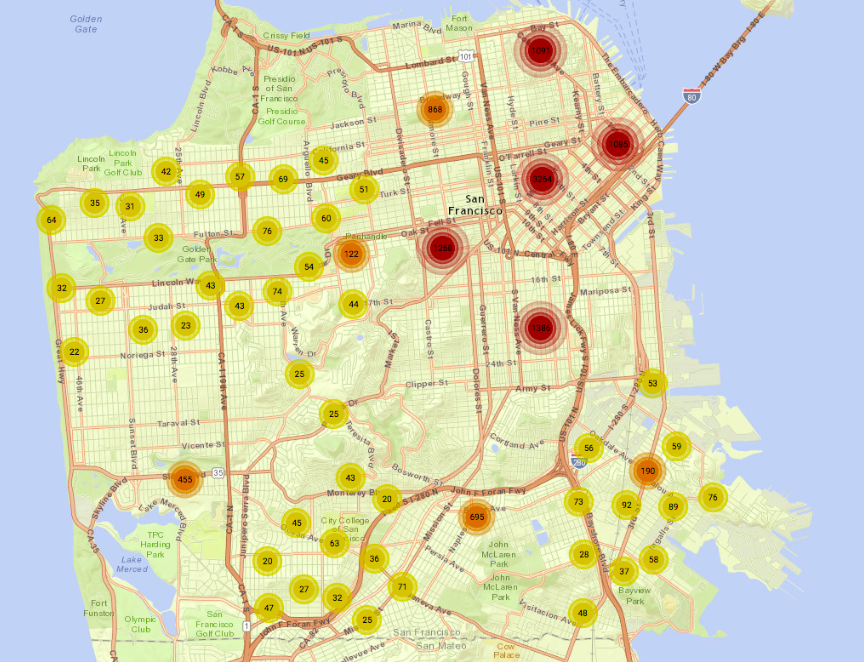
\includegraphics[width=0.4\textwidth]{figs/sub_sf_crime_July2015.png}
  \caption{Crime rates in San Francisco\label{fig:sf_crime}}
\end{figure}

Formally, let $\cU$ be the uploaded auxiliary dataset of lat-long pairs, 
$N=(x_N,y_N)$ a node in our planner and $r$ the effective radius.
We first compute the set $\cP \subseteq A$ of auxiliary points such that,
for every node $P \in \cP$, the Euclidean distance between $N$ and $P$
is within $r$.
Then, the score of auxiliary data for $N$ with respect to $\cP$ and $r$,
denoted by $S(N,\cP,r)$, is computed as follows.

\begin{equation*}
	S(N,\cP,r) = \sum_{\substack{P \in \cP}} 
		\Big(1 - \frac{\sqrt{(x_N-x_P)^2+(y_N-y_P)^2}}{r}\Big)
\end{equation*}

Now we turn to \figref{aux} for an instance to show how auxiliary data
are integrated into the graph using the equation above.
In \figref{aux}, we have the green nodes denoting the graph nodes, 
and the red nodes the new auxiliary nodes that represent locations
of criminal events.
For node $N$, there are three red nodes within its neighborhood of
radius of $r$; thus, we have $\cP=\{P_1,P_2,P_3\}$.
We assume $r$ is 100 feet, and the distances from $N$ to $P_1$,
$P_2$ and $P_3$ are 25, 80 and 90 feet, respectively.
Then, the crime score of $S(N,\cP,r)$ is $1.05$.

\begin{figure}[!ht]
  \centering
    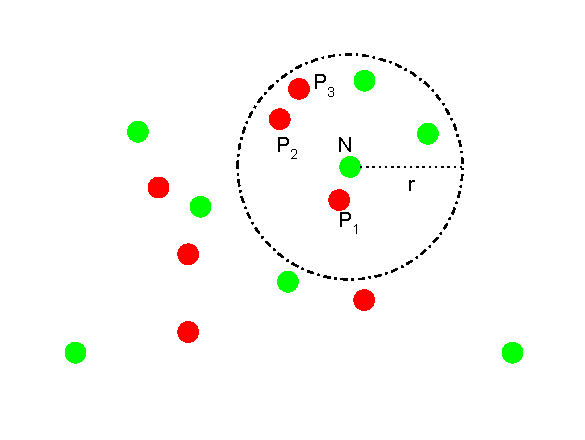
\includegraphics[width=0.4\textwidth]{figs/aux.pdf}
  \caption{Integrating uploaded data\label{fig:aux}}
\end{figure}
